
\title{Opening the Black Box of\\Deep Neural Networks via Information}
\subtitle{Section 2: Information Theory of Deep Learning}
\author{Ravid Shwartz-Ziv \and Naftali Tishby}
\date{}


{\setbeamertemplate{footline}{}
\begin{frame}[plain]
  \vspace{0.8cm}
  \titlepage
  \vfill
  {\color{Accent}\rule{2.2cm}{2pt}}
\end{frame}
}

\begin{frame}{Problem and intuition}
  \begin{columns}[T,onlytextwidth]
    \column{0.46\textwidth}
      {\color{Accent}\large The problem}\par
      \vspace{0.18cm}
      Can we understand the relationship between prediction error and model complexity through the lens of information theory

    \column{0.46\textwidth}
      {\color{Teal}\large The paper's proposal}\par
      \vspace{0.18cm}
      Track each hidden layer through two questions:
      \begin{itemize}
        \item How much input information remains?
        \item How much label information remains?
      \end{itemize}
  \end{columns}
  \vfill
  \centering
  \begin{beamercolorbox}[wd=0.88\textwidth,sep=0.32cm,center]{block body}
  \end{beamercolorbox}
\end{frame}

% TODO change H -> T H confuses with entropy

\begin{frame}{Mutual information}
  \begin{columns}[T,onlytextwidth]
    \column{0.44\textwidth}
      {\color{Accent}\large Definition}\par
      \vspace{0.2cm}
      \[
        I(A;B)=H(A)-H(A\mid B)
      \]
      Observing $B$ is useful when it reduces uncertainty about $A$.

    \column{0.50\textwidth}
      {\color{Teal}\large The two quantities we need}\par
      \vspace{0.22cm}
      \textbf{$I(X;T)$: input information}\par
      How much can the representation $T$ tell us about the input $X$?
      \vspace{0.45cm}

      \textbf{$I(T;Y)$: label information}\par
      How much can the representation $T$ tell us about the target $Y$?
  \end{columns}
  \vfill
  \centering
  {\color{Muted}\small Mutual information is zero when the variables are independent and increases as they share more information.}
\end{frame}

\begin{frame}{The Information Bottleneck Method}
  \centering
  {\color{Muted}\small Introduced by Tishby, Pereira, and Bialek in
  \emph{The Information Bottleneck Method} (1999).}
  \vspace{-0.05cm}
  \[
    \boxed{
      \min_{p(t\mid x)}
      \left[
        \underbrace{\mutualinfo{X}{T}}_{\text{representation complexity}}
        - \beta\,
        \underbrace{\mutualinfo{T}{Y}}_{\text{predictive fitness}}
      \right]
    }
  \]
  \vspace{0.35cm}
  \begin{columns}[T,onlytextwidth]
    \column{0.46\textwidth}
      \centering
      {\color{Accent}\large Compress}\par
      \vspace{0.15cm}
      Discard details of $X$ that do not help predict $Y$.
    \column{0.46\textwidth}
      \centering
      {\color{Teal}\large Predict}\par
      \vspace{0.15cm}
      Preserve the information in $T$ that is useful for predicting $Y$.
  \end{columns}
  \vspace{0.35cm}
  $\beta$ controls how strongly predictive fitness is valued relative to compression.\par
  \vspace{0.12cm}
  {\color{Muted}\small This is a theoretical representation objective, not the
  network's cross-entropy loss. Varying $\beta$ traces the optimal IB frontier.}
\end{frame}

\begin{frame}{The information plane}
  \centering
  {\small
    The network induces the Markov chain
    $Y\!\longleftarrow\!X\!\longrightarrow\!T_1\!\longrightarrow\!\cdots
    \!\longrightarrow\!T_n\!\longrightarrow\!\hat{Y}$.}
  \vspace{0.1cm}
  \begin{columns}[c,totalwidth=0.94\textwidth]
    \column{0.46\textwidth}
      \centering
      \resizebox{\linewidth}{!}{%
      \begin{tikzpicture}[x=0.72cm,y=0.72cm,>=Latex]
        \draw[->,thick,Ink] (0,0) -- (6.1,0)
          node[below right] {$\mutualinfo{X}{T}$};
        \draw[->,thick,Ink] (0,0) -- (0,4.6)
          node[above left] {$\mutualinfo{T}{Y}$};
        \draw[Accent,very thick]
          (0.35,0.25) .. controls (1.2,2.1) and (3.0,3.55) .. (5.55,4.0);
        \node[Accent,above] at (3.9,3.85) {optimal IB frontier};
        \draw[Teal,very thick,->] (5.25,0.8) -- (5.05,2.95);
        \draw[Teal,very thick,->] (5.05,2.95) -- (3.15,3.25);
        \fill[Teal] (5.25,0.8) circle (2.5pt);
        \fill[Teal] (5.05,2.95) circle (2.5pt);
        \fill[Teal] (3.15,3.25) circle (2.5pt);
        \node[Teal,right] at (5.25,1.55) {fit};
        \node[Teal,below] at (4.05,3.05) {compress};
      \end{tikzpicture}
      }
    \column{0.48\textwidth}
      Each hidden layer is one point:
      \[
        \left(I(X;T),\,I(T;Y)\right).
      \]
      \textbf{Upward:} retain more label information.\par
      \vspace{0.18cm}
      \textbf{Leftward:} retain fewer input details.\par
      \vspace{0.3cm}
      {\small The frontier is an optimum. A trained layer is not guaranteed to lie on it.}
  \end{columns}
  \vspace{0.08cm}
  {\color{Muted}\small By the data-processing inequality, later layers cannot recreate information discarded by earlier processing.}
\end{frame}

% \begin{frame}{Main claims}

% \begin{itemize}
%     \item Most of training time is spent compressing, not fitting
%     \item Compression begins when training error saturates
%     \item Converged layers sit on (or very near) the theoretical IB bound
%     \item Adding hidden layers dramatically reduces training time
%     \item Hidden layers are expected to converge near critical points on the IB curve
% \end{itemize}
    
% \end{frame}

\begin{frame}{The role of noise}
\begin{itemize}
    \item \textbf{Core problem}:
    MI is blind to complexity when the map is deterministic \\ 
    %MI is invariant to any invertible relabeling of X — this is why a deterministic f is invisible to $I(X;Y)$
    If Y is a deterministic function of X $(y=f(x))$, then $H(Y|X=x)= 0$ $\forall x$ \\ and:
    $$I(X;Y)=H(Y) - H(Y|X) \quad \Rightarrow \quad I(X;Y) = H(Y)$$  
    %%%%
    \item \textbf{Solution:} \\
    Replace the hard label with a soft, margin-dependent one using a sigmoidal function:
    $$ p(y=1\mid x) = \psi\big(w \cdot x), \qquad \psi(u) = \frac{1}{1+\exp(-\gamma u)}$$
    %where $\theta$ is chosen so $p(y=1)\approx 0.5$ and $\gamma$ tuned so $I(X;Y)\approx 0.99$ bits.
    \begin{itemize}
        \item Points near the boundary are genuinely ambiguous
        \item Points far away are confident
        \item So $I(X;Y)$ now depends on the margin distribution — i.e., on the rule's geometry.
    \end{itemize}
\end{itemize}

\end{frame}

\begin{frame}{Experimental setup}

\begin{itemize}
    \item Synthetic binary classification problem
    \item 12 binary inputs $\Rightarrow 2^{12} = 4096$ possible input patterns
    \item Binary target label $Y \in \{0,1\}$ soften with rule from last slide
    \item Fully connected DNN, trained with SGD and cross-entropy
    \item tanh as hidden activations and sigmoid as output
    \item No explicit regularization
\end{itemize}

\vspace{0.16cm}

\centering
\textbf{For each hidden layer $T_i$:}

\vspace{0.12cm}

\begin{columns}[T,onlytextwidth]
  \column{0.46\textwidth}
    \centering
    $I(X;T_i)$\\
    {\small input information / representation complexity}
  \column{0.46\textwidth}
    \centering
    $I(T_i;Y)$\\
    {\small label information / predictive fitness}
\end{columns}

\vspace{0.22cm}
{\small\color{Muted}
Each scalar activation is assigned to one of 30 bins, creating a many-to-one
mapping. Without quantization, deterministic activations would give
$I(X;T_i)=H(X)=12$ bits throughout training.}
\end{frame}


\begin{frame}{Main result: two phases of training}
\begin{columns}[c,onlytextwidth]
\begin{column}{0.61\textwidth}
    \centering
    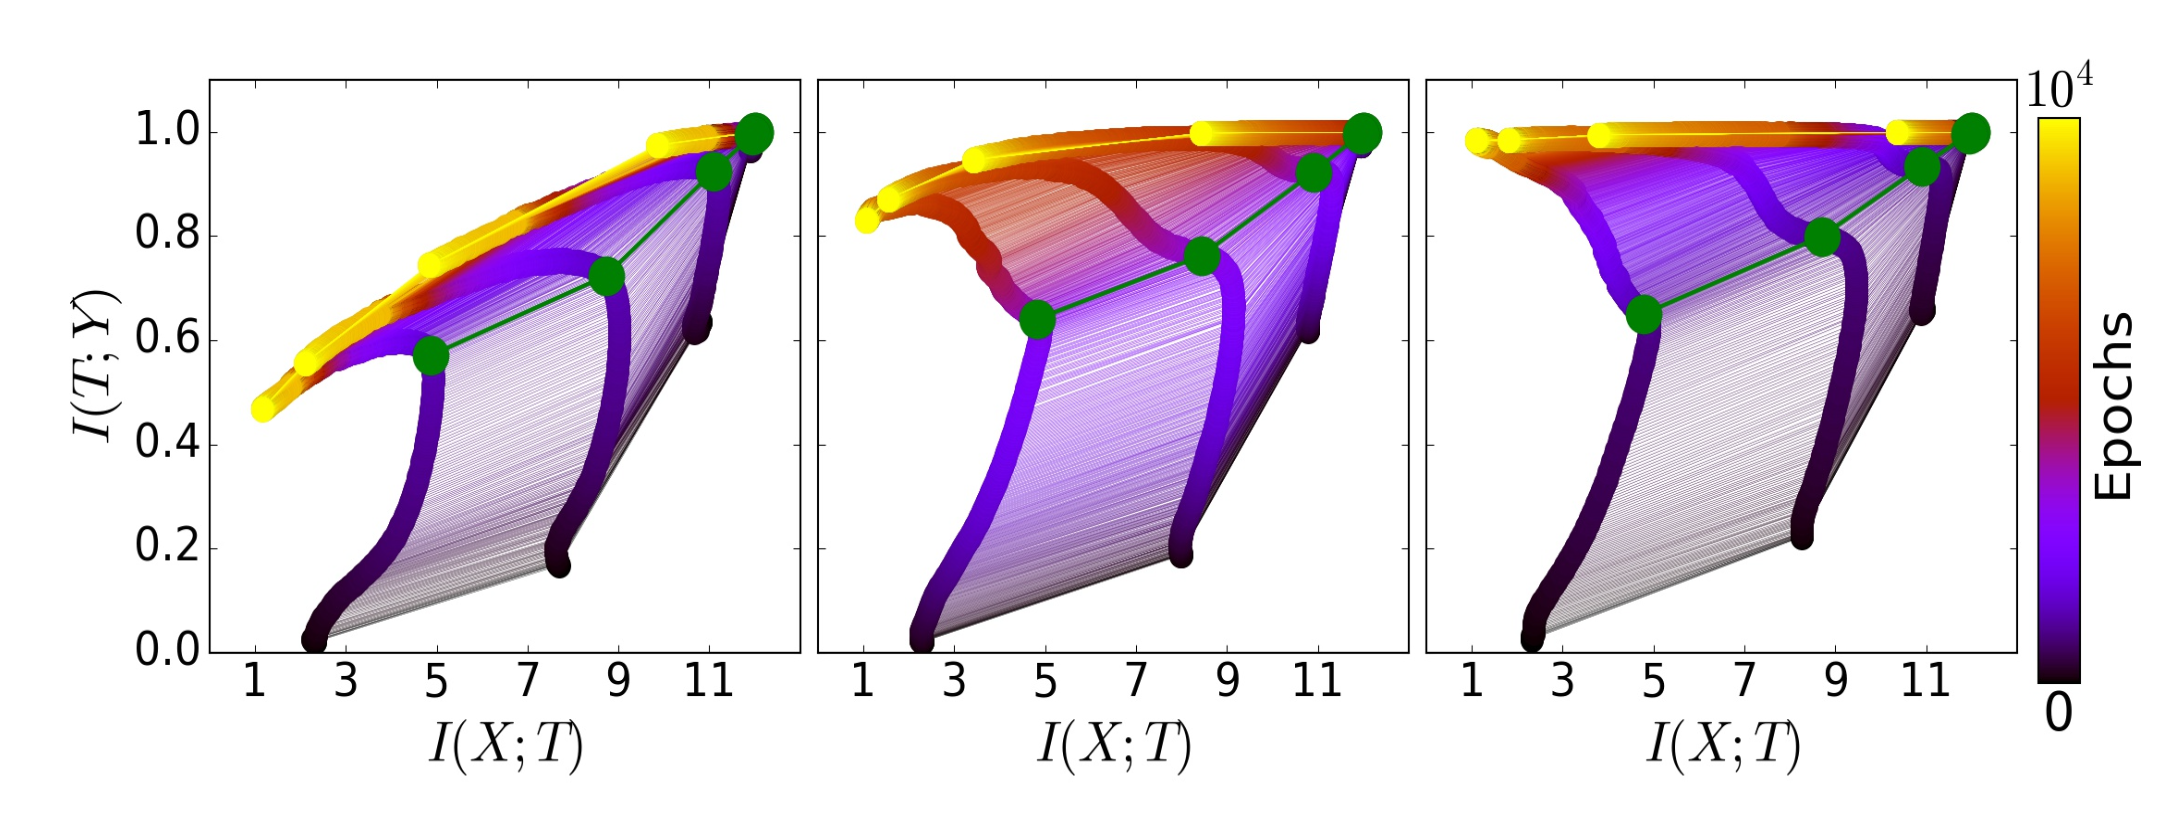
\includegraphics[width=\textwidth,height=0.59\textheight,keepaspectratio]{figures/figure3.png}
\end{column}
\begin{column}{0.36\textwidth}
{\color{Accent}\large Phase 1: Fitting}\par
\vspace{0.15cm}
$I(T;Y)$ rises quickly and gradient mean is large, but variance is small.
\vspace{0.5cm}

{\color{Teal}\large Phase 2: Compression}\par
\vspace{0.15cm}
$I(X;T)$ falls slowly and gradient variance is larger.
\end{column}
\end{columns}
\end{frame}

\begin{frame}{What does depth change?}

\begin{columns}

\begin{column}{0.62\textwidth}
    \centering
    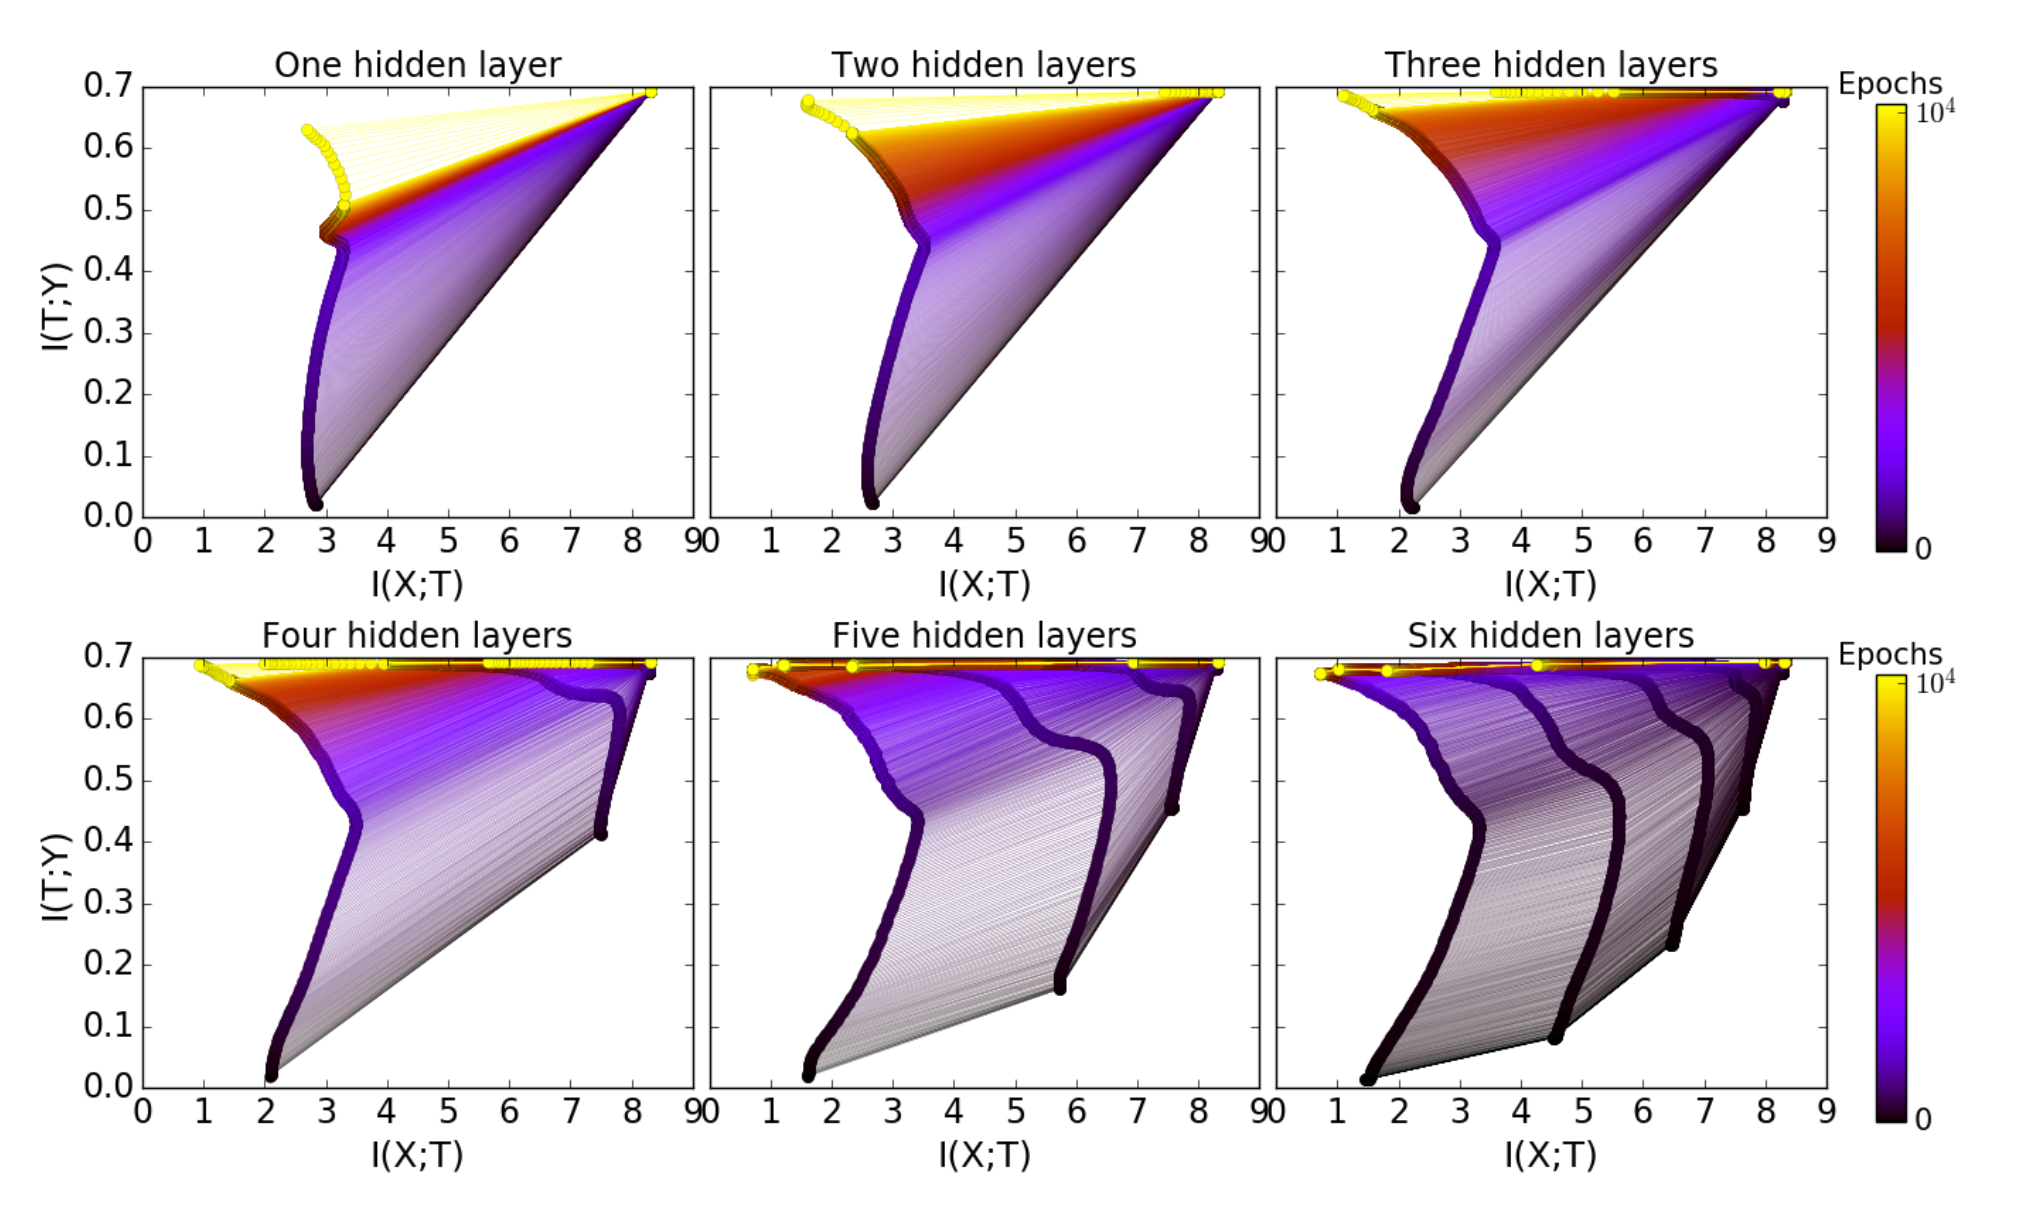
\includegraphics[width=\textwidth]{figures/figure5.png}
\end{column}

\begin{column}{0.38\textwidth}
\begin{itemize}
    \item Increasing depth substantially reduces the number of epochs needed to reach high $I(T;Y)$.
    \item During compression, deeper layers converge before the layers closer to the input.
    \item A compressed predecessor makes the next layer's compression easier.
\end{itemize}
\end{column}

\end{columns}

\end{frame}

\begin{frame}{Discussion: Compression $\Rightarrow$ Generalization?}

\begin{itemize}
    \item What tools did this paper provide, to analyze the fitness and complexity of a model?
   % Tool: measure everything in bits. Per-hidden layer two numbers i.e. dots on a plane. (bits about label and input).
   % Information Bottleneck as reference curve, theoretical bound, and gap to optimal.
   % Invariant to weights. Two phases: fitting then compression.
   % Candidate complexity I(X; T) -- representation/activations not weights
    \item[-]
    \item[-] 
    \item[-]
    \item[-] 
    \item[-] 
\end{itemize}

\end{frame}

\begin{frame}{Discussion: Compression $\Rightarrow$ Generalization?}

\begin{itemize}
    \item What tools did this paper provide, to analyze the fitness and complexity of a model?
    \item To what do they claim the generalization capabilities of DNN is owed?
    % They believe that compression occurs with SGD and this is responsible for absence of overfitting in DL. 
    % They say it generates highly efficient internal representation through compression by diffusion.
    \item[-] 
    \item[-] 
    \item[-] 
\end{itemize}

\end{frame}

\begin{frame}{Discussion: Compression $\Rightarrow$ Generalization?}

\begin{itemize}
    \item What tools did this paper provide, to analyze the fitness and complexity of a model?
    \item To what do they claim the generalization capabilities of DNN is owed?
    \item SGD noise $\rightarrow$ diffusion $\rightarrow$ minimizes $I(X;\;T_i)$ $\rightarrow$ fewer bits about input $\rightarrow$ generalization.
    Is compression generalization?
    % They give a lot of methods and thought into the two phases and the curious role of SGD. They sort of let it be implicit that DNNs generalize, and that compression is the key. Popular school of thought: compression is learning. But what evidence do they provide that compression is learning?
    \item[-] 
    \item[-] 
\end{itemize}

\end{frame}

\begin{frame}{Discussion: Compression $\Rightarrow$ Generalization?}

\begin{itemize}
    \item What tools did this paper provide, to analyze the fitness and complexity of a model?
    \item To what do they claim the generalization capabilities of DNN is owed?
    \item SGD noise $\rightarrow$ diffusion $\rightarrow$ minimizes $I(X;\;T_i)$ $\rightarrow$ fewer bits about input $\rightarrow$ generalization.
    \item Are their methods scalable?
    % Compression-is-learning is a whole school. But what evidence HERE? They show compression happens and that label info survives -- never that the compression caused the generalization.
    % No test error plotted anywhere. Compression is potentially just correlated.
    \item[-] 
\end{itemize}

\end{frame}

\begin{frame}{Discussion: Compression $\Rightarrow$ Generalization?}

\begin{itemize}
    \item What tools did this paper provide, to analyze the fitness and complexity of a model?
    \item To what do they claim the generalization capabilities of DNN is owed?
    \item SGD noise $\rightarrow$ diffusion $\rightarrow$ minimizes $I(X;\;T_i)$ $\rightarrow$ fewer bits about input $\rightarrow$ generalization.
    \item Are their methods scalable?
    \item Complexity is measured as MI over binned activations. Does that measure the network, or the binning? (Saxe et al. '18)
\end{itemize}

\end{frame}

\begin{frame}{Discussion: Compression $\Rightarrow$ Generalization?}

\begin{itemize}
    \item What tools did this paper provide, to analyze the fitness and complexity of a model?
    \item To what do they claim the generalization capabilities of DNN is owed?
    \item SGD noise $\rightarrow$ diffusion $\rightarrow$ minimizes $I(X;\;T_i)$ $\rightarrow$ fewer bits about input $\rightarrow$ generalization.
    \item Are their methods scalable?
    \item Complexity is measured as MI over binned activations. Does that measure the network, or the binning? (Saxe et al. '18)
    % Their I(X;T) can only move because tanh outputs get chopped into 30 bins -- the net is deterministic and X is discrete, so information-theoretically the layer keeps all 12 bits forever. "Compression" = inputs saturating toward +-1 and collapsing into shared bins. Saxe's three blows: (1) swap tanh for ReLU and compression largely disappears -- generalization unaffected; (2) full-batch GD, no minibatch noise, still compresses -- kills the diffusion mechanism; (3) they construct cases where compression and generalization move independently. So the phenomenon is a property of double-saturating nonlinearities plus a discretization choice, not of learning. Note the irony: paper's own S2.4 argues MI is meaningless for deterministic nets and you need noise -- then runs deterministic nets and lets the binning stand in for the noise ###CLAUDE GENERATED ###
\end{itemize}
\end{frame}